\subsection{Usage Behavior}
\label{subsec:behavior}

We estimate the mean spacio-temporal usage behavior of a household by aggregating broadband data transferred every 15 mins for each device over each day.

\todo{make two sub plots for (a) test and (b) control: (mean of day) (sum of device) bytes, include (perc90 of day) (sum of device) bytes and (median of day) (sum of device) bytes. Purpose is to show patterns individually, not compare differences. Patterns to show are (1) no troughs in usage, (2) prime-time hours shift (subsection ~\ref{subsec:primetime}), (3) difference between 90\%-ile and median (subsection ~\ref{subsec:peakratio})}

\todo{separate subplots for M-F and S/S/holidays -- choose two interesting ones}
%We characterize \textbf{usage behaviors} and show that aggregate
% network usage seen by the ISP does not show a trough in the middle
% of the day for high capacity tiers.
%, as observed by aggregate usage across all tiers. % This motivates 
%the need to study usage per tier separately as usage behavior differs
% with tiers.

Based on previous findings, we analyzed weekly patterns and confirmed that households have a higher variance in daily network usage during evenings on weekdays as compared to weeknights and holidays. We thus divide our analysis based on weekday and show show the daily mean, median, and 90-\%ile of the total data rate as seen by the ISP for households the \control and \test sets in figure~\ref{fig:TS-data-rate-daily}. We find that the daily usage behavior on the weekend and holiday usage has four parts: (a) an initial sharp rise, (b) a flatter rise, (c) sharp rise to evening, (d) sharp decrease after 12 am.
In contrast, weekdays have two simple parts: (a) a rise in data usage from 7:00 AM that peaks in late evening around 8:00 PM, and (b) a sharp fall in usage from 12:00 PM to 6:00 AM in the morning. This is in contrast to the widely expected usage patterns network usage patterns analyzed after aggregation at ISPs that show a local small peak in network load in the morning (10AM), then dip in the afternoon, and then rise up again in the late evening ~\cite{sandvine2014report1}, \todo{check if dasu shows this, check other studies.}

\todo{also, test set seems to have this small peak and a trough, but control doesn't. Why??. Also test and control medians differ during office hours (10:00 AM to 6:00 PM) but are similar in peak hours...}
%see: http://sites.noise.gatech.edu/~sarthak/files/comcast/plots/full_dw/describe-total-throughput-per-day-ALL.png

This lack of troughs could be the result of the users' behavior in higher tier bandwidth, and motivated us  to further study user taxonomy in section~\ref{subsec:peakratio}.

%%%%%%%%%%%%%%%%%%%%%%%%%%%%%%%%%%%%%%%%%%%%%%%%%%%%%%%%%%%%%%%%%%%%%
\begin{figure}[ht!]
\begin{minipage}{\linewidth}
  \centering
  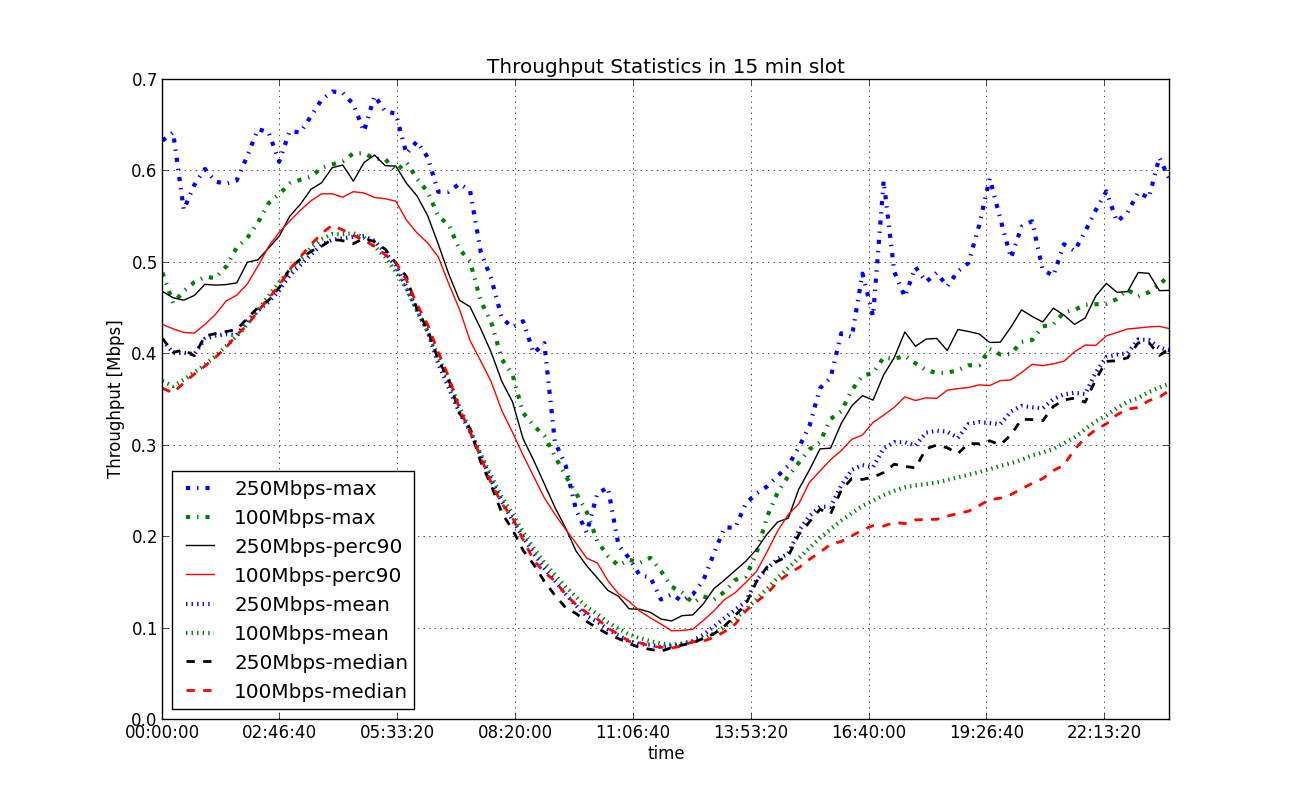
\includegraphics[width=\linewidth]{figures/describe-total-throughput-per-day[replace].png}
  \caption{agg (days) over means (devices): aggregate has no trough, peaks in the evening hours}
  %http://riverside.noise.gatech.edu:8083/separated/full/describe-total-throughput-per-day.png
  \label{fig:TS-data-rate-daily}
\end{minipage}
\end{figure}